\documentclass[11pt, a4paper]{article}
\usepackage{natbib}
\usepackage{eso-pic}
\usepackage{amsmath} % flere matematikkommandoer
\usepackage{amssymb}
\usepackage[utf8]{inputenc} % æøå
\usepackage[T1]{fontenc} % mere æøå
\usepackage[danish, english]{babel} % orddeling
\usepackage{verbatim} % så man kan skrive ren tekst
\usepackage{graphicx}
\usepackage{booktabs}
\usepackage{enumitem}
\usepackage{placeins}
\usepackage[colorlinks=false]{hyperref}
\usepackage{tocbibind}

\author{
    Christian Kjær Larsen \texttt{(011292)} \\[.4cm]
    Lukas Svarre Engedal \texttt{(210790)} \\[.4cm]
    Tobias Sønderskov Hansen \texttt{(240395)} \\[.4cm]
    Instruktor: Aske Mottelson\\[.4cm]
    \vspace{9cm}
}

\title{
  \vspace{3cm}
  \Huge{PoP-Webhelp} \\[.10cm]
  \Large{Delrapport 2, ProjDat 2015}
}

\begin{document}
\selectlanguage{danish}
\AddToShipoutPicture*{\put(0,0){\includegraphics*[viewport=0 0 700 600]{includes/nat-farve}}}
\AddToShipoutPicture*{\put(0,602){\includegraphics*[viewport=0 600 700 1600]{includes/nat-farve}}}

%% Change `ku-en` to `nat-en` to use the `Faculty of Science` header
\AddToShipoutPicture*{\put(0,0){\includegraphics*{includes/nat-en}}}

\clearpage\maketitle
\thispagestyle{empty}

\newpage

\selectlanguage{english}
\begin{abstract}
This report presents the development of an e-learning system for use in the newly created introductory computer science course at the Institute of Computer Science at the University of Copenhagen, called \emph{Programmering og Problemløsning}. Our clients are Martin Dybdal and Oleksandr Shturmov, both employed at the institute, who will be in charge of the course. In the course, the students will be taught the programming language \verb!F#!.

The aim of the e-learning system is to introduce new students to programming in a simple and user-friendly way, and to teach them various basic ideas and concepts in programming in general, and \verb!F#! in particular. This is done by presenting the students with an array of different exercises, sorted based on subject and difficulty, and presented to students in a specific and meaningful order.

The system will have two different kinds of users: students and admins.

Students will mainly be working on the various exercises, and they will also be able to get hints for the exercises if needed and provide feedback on the exercises and hints once completed. Students should also be able to see how well they are doing so far, for instance how many of the exercises belonging to a particular subject matter they have solved.

The primary role of the admins will be managing the exercises and supervising how well the students are doing. They should be able to easily delete or modify existing exercises or add new ones, as well as manage the order in which the students are presented with the exercises. They should also be able to get various statistics about how the students are doing in order to improve and optimize the exercises, their order and their subjects.
\end{abstract}
\newpage
\tableofcontents

\thispagestyle{empty}

\newpage
\pagestyle{plain}
\setcounter{page}{1}
\pagenumbering{arabic}

\selectlanguage{danish}
\section{Review}

\subsection{No Silver Bullet -- Essence and Accident in Software Engineering}
\label{sub:no_silver}

I artiklen \cite{nsbullet} beskriver Brooks nogle af de barrierer der skal forceres før vi kan få betydelige produktivitetsforbedringer inden for softwareudvikling. Han sammenligner det med Moores lov, men siger at det er urealitisk at ville kunne se de samme fremskridt som inden for hardware. Brooks nævner først den store kompleksitet i software som en af de helt store udfordringer. Det at kompleksiteten ved software ofte stiger eksponentialt med projektets størrelse er problematisk. Dette gør det også sværere at vedligeholde, og hvis der er mange der arbejder på projektet samtidigt, så kan det blive svært at koordinere. Han mener også, at i forhold til andre produkter som er mere fysiske, så er der ikke en entydig måde at visualisere software på, og det bliver derved også svært at overskue.

Senere i artiken forklarer Brooks om hvilke fremsridt der allerede er gjort inden for softwareudvikling, som har gjort det mindre komplekst. Han nævner ting som højniveausprog, operativsystemer og overgangen fra batch-processer til \emph{time-sharing}, altså det at man kan køre flere programmer på en gang, som nogle af de vigtige fremskridt.

Han fortsætter med at skrive om nogle af hans forhåbninger til den nærmeste fremtid. Han skriver især om de forhåbninger han har omkring nøjniveausprog. Han nævner blandt andet muligheder for modularisering af programmer i sproget Ada, og de fremskridt der sker inden for objektorienteret programmering. Han ser dog ikke nogen mulighed for produktivitetsforbedringer på en hel størrelsesorden. Nogle af de ting han ikke har så meget tiltro til er nogle af det mere automatiske kodeværktøjer. Det kan fx være grafiske værktøjer, hvor man tegner flowcharts for at beskrive kontrolflowet i programmet. Han begrunder sin kritik med, at software ikke kan projekteres på et grafisk plan. Han mener at software er multidimensionelt, og meget af kompleksiten skal abstraheres væk på andre måder.

Han slutter artiklen af med nogle af de idéer han spår en god fremtid inden for softwareudvikling. Han er især begejstret for analogien med at gro software. Altså det med at kan ikke fra starten har en stor kravspecifikation, og så bagefter bare skriver kode til man er færdig, men i stedet inkrementelt udvikler både software og krav. Han nævner det også som motiverende at se en prototype virke, og det er bedre for kunden at kunne se et fungerende system, og derved kunne træffe beslutninger om udviklingsprojektets retning derefter.

Det er ret utroligt at en artikel skrevet i 1983 kan være så præcis i sin beskrivelse af softwareudvikling, selv mere end tredive år senere. Det er stadig mange af de samme problemer der går igen, og gør softwareudvikling til en besværlig og kompliceret affære. Det er stadigvæk ting som upræcise og konstant skiftende kravspecifikationer der gør at der er mange forfejlede og dyre softwareprojekter.

Der er dog sidenhen kommet flere løsningforslag, der påstår at have hjulpet til at gøre softwareudvikling til en mere forudsigelig proces. En af disse processer som afhjælper nogen af de problemer som Brooks nævner er \emph{Unified Process} (Kapitel 15 i \cite{OOSE}). Den prøver at være drevet af iterationer, samtidig med at man prøver at mindske udviklertimer ved at bruge eksterne moduler som enten kan være frit tingængelige eller som købes.

Senere er der så kommet hele det agile paradigme, hvor man prøver helt at nytænke måden man udvikler software, hvor man nærmest prøvet at omfavne de hurtigt ændrende krav til produktet. Det er metodikker som \emph{SCRUM}\cite{sutherland2010jeff}, \emph{Extreme Programming}\cite[]{OOSE}, kapitel 16.

Der er også sket udvikling inden for værktøjer, som har gjort programmører mere produktive. Det er her værktøjer som integrerede udviklingsmijøer som \emph{Visual Studio} til \verb!.NET! platformen og \emph{IntelliJ} til \verb!Java! som har aflastet programmører i at overskue store kodebaser med enorm kompleksitet. Her er også funktioner til refaktorering, aflusning med flere. Programmeringssprog er også blevet mere højniveau, og der er kommet flere dynamiske sprog som Python, Ruby og Javascript som påstår at højne produktiviteten.

\newpage
\subsection{The M.A.D. Experience: Multiperspective Application Development in evolutionary prototyping}
Artiklen beskriver en overordnet objektorienteret systemudviklingsmetode med fokus på hurtig fremstilling af prototyper, og hvordan denne metode er blevet anvendt i et større projektforløb. Metoden bygger på erfaringer som en forskningsgruppe gjorde sig i forbindelse med en produktudvikling de lavede i samarbejde med et dansk containerrederi.

\emph{Multiperspective} i navnet refererer til tre generelle grupperoller, som hver bidgrager med deres unikke perspektiv til projektet. 
\emph{The ethnographer} fokuserer på den nuværende praksis inden for det område hvor systemet skal bruges. Generelt har M.A.D. metoden gennem hele projektet stort fokus på at designe et produkt der passer ind i den eksisterende praksis, etnografernes analyse spiller derfor en central rolle, da den danner fundament for mange af de andre udviklingsaktiviteter. \emph{Participatory designer}-rollen fokuserer på at inddrage de fremtidige brugere af systemet i designprocessen. Dette gøres ud fra både et moralsk og et praktisk standpunkt. Det er brugerne selv der skal leve med konsekvenserne af de forskellige designbeslutninger. Samtidig antages det at erfaringen fra deres arbejde med det eksisterende system gør dem i stand til at komme med fornuftig respons til designet. I M.A.D. ses design i høj grad som en fællesaktivitet. Sidst er der \emph{OO developer}-rollen som fokuserer på at lave og implementere selve modellen. Disse roller skal ikke forstås som skarpt adskildte, idéen er at de skal komplementerer hinanden.

Der fremhæves tre vigtige erfaringer forfatterne gjorde sig inden for objekt orienteret udvikling: \emph{Analyse er mere end bare at finde navneord}, \emph{design er mere end at udfylde detaljerne i en objektorienteret analysemodel} og \emph{implementering er mere end oversættelse af design modeller til kode}.

Artiklen er fra 1998, siden da er der altså sket betydelige fremskridt inden for software og hardware. På trods af dette er den grundlæggende problematik inden for systemudvikling den samme, og artiklen er da stadig relevant i dag. Da det er en objektorienteret metode inkorporerer den mange af de typiske elementer. Tilføjning af ny funktionalitet skal være let hvilket opnås ved at opbygge systemet efter \emph{model-view-control}, \emph{entity-boundary-controller}, eller et lignende design mønster. Som i så mange andre metoder sker udviklingen i M.A.D. i flere iterationer. Særligt ved metoden beskrevet i artiklen er dog at de overordnede udviklingsaktiviteter \emph{analyse, design} og \emph{implementering} alle udføres parallelt, i modsætning til sekventielt som er typisk for andre fremgangsmåder. Tanken bag dette er at enhver af de tre aktiviter kan gøre brug af erfaring fået under de to øvrige aktiviteter.

Projektet som danner grundlag for artiklen er, i forhold til vores IT-projekt, i meget stor skala, hvilket også gør at der ikke uden videre kan laves en direkte sammenligning mellem de to. Selvom de to projekter er meget forskellige, kan der dog sagtens drages paralleller mellem metoden præsenteret i artiklen og den fremgangsmåde vi har benyttet os af i vores projekt, bl.a. den iterative fremgangsmåde og det tidlige brugerfokus, som agile metoder er kendetegnet ved.

Som nævnt tidligere lægger metoden stor vægt på analyse af den nuværende praksis. Der er dog projekter hvor en sådan nuværende praksis ikke eksisterer. Dette kan siges at være tilfældet i vores projekt, da det produkt vi udvikler ikke skal erstatte noget eksisterende system. I vores tilfælde er der altså visse dele af M.A.D. metoden der ikke ville være nær så relevant.

\newpage
\section{Formål og rammer}
\label{sec:formal_og_rammer}
I dette afsnit beskrives systemets formål og rammer ved \textit{FACTOR}-kriteriet.
\paragraph{Funktionalitet}
\begin{itemize}
    \item Besvare programmeringsspørgsmål
    \item Oprette programmeringsspørgsmpl
    \item Analysere det studerendes fremskridt
    \item Håndtere de studerendes login
\end{itemize}
\paragraph{Anvendelsesområde}
\begin{itemize}
    \item Undervisere ved DIKU
    \item Førsteårsstuderende ved DIKU
\end{itemize}
\paragraph{Betingelser}
\begin{itemize}
    \item Undervisere har begrænsede resurser
    \item Det skal foregå online
\end{itemize}
\paragraph{Teknologi}
\begin{itemize}
    \item Python 2
    \item Flask webframework
    \item SQLAlchemy
    \item HTML/CSS
    \item Javascript
\end{itemize}
\paragraph{Objekter}
Studerende, Spørgsmål, Hint, Underviser.
\paragraph{Ansvar}
E-læringssystem der skal hjælpe de studerende med programmering.

\section{Kravspecifikation}
\label{sec:kravspecifikation}
I dette afsnit beskrives kravene til systemet. Det er ting som de funktionelle og de ikke-funktionelle krav til systemet. Der er også diagrammer der uddybber systemets funktionalitet og udformning.
\subsection{Krav}
\label{sub:krav}
\paragraph{Funktionelle krav}
De funktionelle krav for systemet er i tråd med afsnit 4.3.1 i \cite{OOSE}, nemlig at de omhandler den specifikke brug af systemet.
\begin{itemize}
    \item Systemet skal være en hjemmeside med opgaver, som kan løses individuelt af studerende.
    \item Der kræves login, så man kan følge med i den studerendes udvikling.
    \item Spørgsmålene skal være grupperede efter hvilke læringsmål de tester.
    \item Læringsmålene skal igen grupperes i nogle blokke, hvor idéen så er at man gennemgår blokkene én af gangen i en bestemt rækkefølge, og at sværhedsgraden stiger løbende.
    \item Der skal være hints til opgaverne som de studerende kan benytte hvis nødvendigt, og de studerende skal så kunne give feedback til hints'ne.
    \item Alle forsøg på opgavebesvarelser skal gemmes i en log.
\end{itemize}
Hvis der er tid i en af de senere iterationer, så er der en række ekstra krav som kan implementeres.
\begin{itemize}
    \item Loggen skal bruges til at give underviseren information om hvilke spørgsmål der er svære.
    \item Der skal tilføjes en grad af \emph{gamification}, så der gives badges og point for fremskridt, og det bliver muligt at følge med i andres fremskridt.
    \item Hvis man ikke har øvet sig i et emne i et stykke tid, så falder ens erfaring i området.
\end{itemize}

\paragraph{Ikke-funktionelle krav}
\label{par:ikke_funktionelle_krav}
I afsnit 4.3.2 i \cite{OOSE} beskrives ikke-funktionelle krav som krav, der ikke direkte beskriver funktionaliteten, men mere generelle krav omkring ting som brugervenlighed, ydeevne, pålidelighed og hvor vedligeholdesesvenligt systemet er.

De ikke-funktionelle krav til dette projekt er forholdsvis begrænsede, idet vi har fået ret stor frihed i forhold til hvordan vi løser opgaven af vores kunde.

\begin{itemize}
\item Det skal være nemt at tilføje nye opgaver til systemet, sådan at kursuslederne efterfølgende kan opbygge en tilstrækkelig samling af opgaver til de studerende.
\item Det endelige produkt skal gerne skal være simpelt og modulært, sådan at det er nemt at overtage, udvide og bygge videre på efter at vi overgiver projektet til kunden.
\item Ingen af kunderne er web-udviklere, så det er også vigtigt at det valgte framework er veldokumenteret og rimeligt simpelt at bruge.
\end{itemize}

\subsection{Use case model}
\label{sub:use_case_model}
På Figur \ref{fig:use_case_model} kan man se vores use case model diagram. Vi har at gøre med to aktører, nemlig studerende og administratorer. Det vigtige for studerende er at de kan oprette sig på siden, og at de har adgang til opgaver de kan besvare. Det vigtige for administratorer er at de kan administrere opgaverne, og at de kan få feedback og statistik på hvordan de studerende klarer opgaverne. Begge aktører skal desuden kunne benytte simpel funktionalitet i forbindelse med deres login.
\begin{figure}[h]
  \centering
  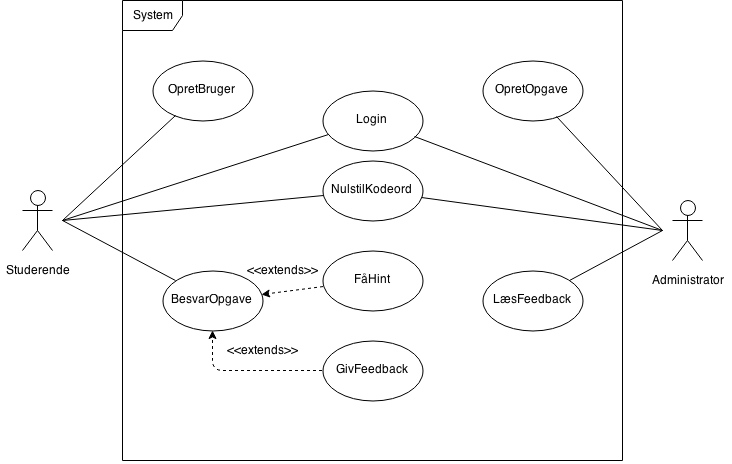
\includegraphics[width=0.8\linewidth]{figures/UseCaseModel.png}
  \caption{Use case model for vores system.}
  \label{fig:use_case_model}
\end{figure}
\subsection{Use cases}
\label{sub:use_cases}

På Figur \ref{fig:use_case1} ses en beskrivelse af use casen, hvor en studerende opretter sin bruger. Det er en simpel use case, der beskriver i detaljer hvordan processen med at oprette sig som bruger i systemet skal foregå. Inden denne use case, så har brugeren ikke oprettet sig, og når use casen er fuldført, så har brugeren oprettet sig, er godkendt og logget ind. Det kombinerer en del af funktionaliteten i én use case. Det kunne godt deles op, men da vi her kun skal beskrive tre overordnede use cases, så har vi kombineret dem.
\begin{figure}[h!]
    \centering
    \begin{tabular}{r p{8cm}}
        \toprule
        \textit{Navn på use-case:} & \verb!OpretBruger! \\
        \hline
        \textit{Deltagende aktører:} & Påbegyndt af en studerende \\
        \hline
        \textit{Hændelser:} & \begin{enumerate}[nolistsep]
            \item En studerende åbner hjemmesiden og klikker på \verb!register!
            \item Den studerende indtaster sine brugeroplysninger, dvs. ku-id og løsen.
            \item Systemet opretter brugeren, og sender en e-mail med et aktiveringslink.
            \item Den studerende klikker på linket, og kontoen aktiveres.
            \item Den studerende bringes til login-siden.
            \item Den studerende indtaster ku-id og løsen og klikker \verb!Login!
            \item Der informeres om succesfuldt login, og brugeren bringes til applikationen.
        \end{enumerate}  \\
        \hline
        \textit{Startbetingelse:} & En studerende har ingen konto, og er ikke logget ind. \\
        \hline
        \textit{Slutbetingelse:} & En studerende har en aktiveret konto og er logget ind. \\
        \bottomrule
    \end{tabular}
    \caption{Use case omkring oprettelse af brugere.}
    \label{fig:use_case1}
\end{figure}

På Figur \ref{fig:use_case2} ses en beskrivelse af use casen, hvor en studerende svarer på spørgsmål. Den er på et relativt højt abstraktionsniveau, da vi ikke er helt sikre på hvordan workflowet i systemet er endnu. En ting er dog sikkert. Når man har valgt et emne, så vil der blive stillet spørgsmål i en lind strøm, indtil systemet finder at man har dygtiggjort sig nok inden for emnet til at man kan begynde på et nyt.
\begin{figure}[h!]
    \centering
    \begin{tabular}{r p{8cm}}
        \toprule
        \textit{Navn på use-case:} & \verb!BesvarOpgave! \\
        \hline
        \textit{Deltagende aktører:} & Påbegyndt af en studerende \\
        \hline
        \textit{Hændelser:} & \begin{enumerate}[nolistsep]
            \item En studerende åbner hjemmesiden.
            \item Vedkommende vælger et emne inden for en læringsblok der er låst op ved at have færdiggjort den forrige.
            \item Systemet præsenterer et spørgsmål for den studerende. Der kan være flere typer spørgsmål (multiple-choice, udfyldning med flere).
            \item Den studerende indtaster et svar.
            \item Systemet giver respons på svaret, og gemmer det i en historik.
            \item Den studerende trykker næste, for at få et spørgsmål mere.
            \item Hvis den studerende har svaret på nok spørgsmål, så kan den studerende vælge en ny kategori.
            \item Den studerende lukker browseren.
        \end{enumerate}  \\
        \hline
        \textit{Startbetingelse:} & En studerende der er logget ind. \\
        \hline
        \textit{Slutbetingelse:} & En studerende der er logget ind og har besvaret en eller flere opgaver. \\
        \bottomrule
    \end{tabular}
    \caption{Use case omkring besvarelse af opgaver.}
    \label{fig:use_case2}
\end{figure}

Et af kravene for systemet er, at det skal være nemt for underviserne i kurset at oprette nye opgaver. Da underviserne selv er dataloger, så vil det være optimalt hvis man kan lave spørgsmålene i et struktureret filformat. Vi har foreslået \verb!YAML!, derfor er use-casen på Figur \ref{fig:use_case3} meget simpel, og består kun af fil-upload.
\begin{figure}[h!]
    \centering
    \begin{tabular}{r p{8cm}}
        \toprule
        \textit{Navn på use-case:} & \verb!OpretOpgave! \\
        \hline
        \textit{Deltagende aktører:} & Påbegyndt af en administrator \\
        \hline
        \textit{Hændelser:} & \begin{enumerate}[nolistsep]
            \item Vedkommende trykker på \verb!Add Question!.
            \item En YAML fil uploades i en formular.
            \item Brugeres informeres om at spørgsmålet er oprettet.
        \end{enumerate}  \\
        \hline
        \textit{Startbetingelse:} & En administrator der er logget ind. \\
        \hline
        \textit{Slutbetingelse:} & En administrator der er logget ind og har oprettet en opgave. \\
        \bottomrule
    \end{tabular}
    \caption{Use case omkring oprettelse af opgaver.}
    \label{fig:use_case3}
\end{figure}

\subsection{Klassediagram}
\begin{figure}[h]
    \centering
    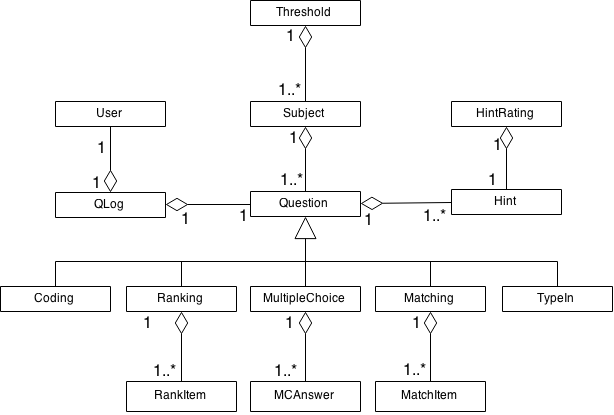
\includegraphics[width=0.8\linewidth]{figures/ClassDiagram.png}
    \caption{Klassediagram af problemområdet}
    \label{fig:class_diagram}
\end{figure}
På Figur \ref{fig:class_diagram} kan man se vores klassediagram. Størstedelen af klasserne har at gøre med opgaverne og deres inddeling i forskellige grupper samt de forskellige typer af opgaver der findes. Derudover er der et par klasser der har at gøre med den log der føres over de studerendes opgavebesvarelser, for at de kursusansvarlige kan følge med i hvad der går godt og mindre godt. Endeligt er der en klasse for studerende og en klasse for administratorne.
\subsection{BCE-model}
\begin{figure}[h]
  \centering
  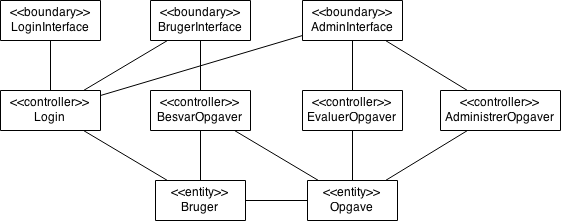
\includegraphics[width=0.8\linewidth]{figures/BCE-Model.png}
  \caption{BCE model for vores system.}
  \label{fig:bce_model}
\end{figure}
På Figur \ref{fig:bce_model} kan man se vores BCE model. Modellen har to entity-objekter, fire controller-objekter samt tre boundary-objekter.

De to entity-objekter er \emph{Bruger} og \emph{Opgave}. \emph{Bruger} indeholder informationer om hver enkelt bruger som login-oplysninger, hvor vidt brugeren er en studerende eller en admin samt hvilke opgaver brugeren allerede har løst. \emph{Opgave} indeholder alle informationerne om de enkelte opgaver, det er både selve opgaven der skal løses samt statistik omkring hvordan det er gået når studerende har løst opgaven.

Modellen har tre boundary-objekter, hvor det første man vil møde når man indlæser siden er \textit{login}-brugergrænsefladen, der sammen med \emph{login}-controlleren sørger for at logge brugerne ind i systemet. Derefter vil man så enten have adgang til \emph{Bruger}-grænsefladen eller \emph{Admin}-grænsefladen afhængig af hvad ens status er, og derfra har man adgang til en række controllers.

Modellen har fire controller-objekter, hvor den første er \emph{login}-controlleren der som tidligere nævnt står for at logge brugere ind i systemet. Som studerende vil man have adgang til \emph{BesvarOpgave}-controlleren, der snakker sammen med \emph{Bruger} og \emph{Opgave} og sørger for at stille brugeren de rigtige opgaver. Som admin vil man have adgang til to controllers, nemlig \emph{EvaluerOpgave}-controlleren og \emph{AdministrerOpgave}-controlleren. \emph{EvaluerOpgave}-controlleren snakker sammen med \emph{Opgave} og giver en adgang til de forskellige slags statistik der bliver samlet om opgaverne, og \emph{AdministrerOpgave}-controlleren snakker ligeledes sammen med \emph{Opgave} og giver en adgang til at slette eller ændre i eksisterende opgaver samt tilføje nye.

\subsection{Sekvens-diagrammer}
I dette afnit er der lavet sekvensdiagrammer over de tre use cases der er beskrevet i Afsnit \ref{sub:use_cases}.
\begin{figure}[h]
    \centering
    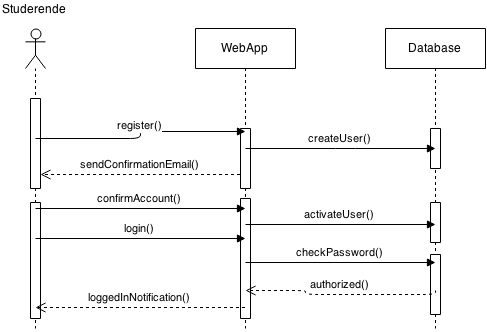
\includegraphics[width=0.8\linewidth]{figures/OpretBrugerUseCase.png}
    \caption{Sekvensdiagram over opretning af bruger}
    \label{fig:opret_bruger_sekvens}
\end{figure}
På Figur \ref{fig:opret_bruger_sekvens} kan man se sekvens-diagrammet for den første use case, der beskriver hvordan en studerende opretter sig som bruger i systemet. Her indgår to adskilte sessioner. En hvor brugeren opretter sig. Så sender systemet en email til brugeren. I næste session klikker brugeren på et link i denne email, og brugeren aktiveres. Derefter logger vedkommende ind. Brugeren gøres opmærksom på at dette er lykkedes, og use casen er færdig.

\begin{figure}[h]
    \centering
    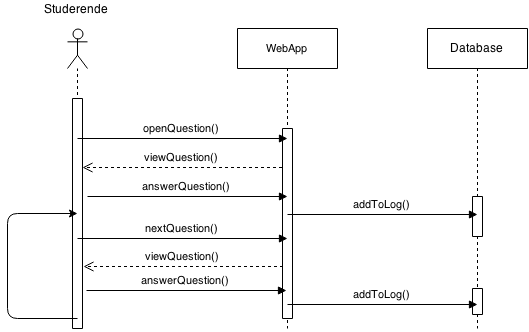
\includegraphics[width=0.8\linewidth]{figures/SvarUseCase.png}
    \caption{Sekvensdiagram over besvarelse af spørgsmål}
    \label{fig:svar_sekvens}
\end{figure}
På Figur \ref{fig:svar_sekvens} kan man se sekvens-diagrammet for den anden use case, der beskriver hvordan en studerende besvarer spørgsmål. Brugeren åbner et spørgsmål, og kan ved at svare kommer videre til næste spørgsmål. Løkken viser at der kan komme flere end et spørgsmål efter det første.

\begin{figure}[h]
    \centering
    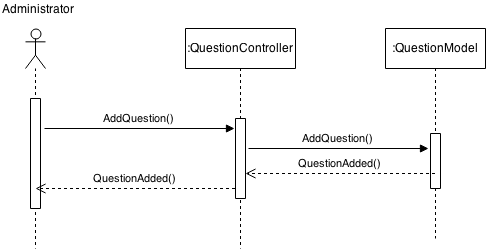
\includegraphics[width=0.8\linewidth]{figures/OpretSporgsmalUseCase.png}
    \caption{Sekvensdiagram over opretning af spørgsmål}
    \label{fig:opret_sp_sekvens}
\end{figure}
På Figur \ref{fig:opret_sp_sekvens} kan man se sekvens-diagrammet for den tredje use case, der beskriver hvordan en administrator opretter et nyt spørgsmål i systemet. Dette sekvensdiagram er stort set linært, da der ikke sker mere ed at der uploades et spørgsmål, og der gives respons på at det er tilføjet korrekt.

\section{Systemdesign}
\label{sec:systemdesign}
I dette afsnit beskrives de designopgaver der er udført allerede. Til sidst i afsnittet vises de dele der endnu ikke er udført.
\subsection{Strukturering}
\label{sub:strukturering}

I nogle udviklingsmiljøer er der typisk givet en struktur af kodebasen på forhånd. Det gælder mange gange når man bruger store frameworks som Django til Python eller Play til Java. Der er nogle konventioner til hvilke klasser der skal i hvilke mapper, og til hvordan konfigurationsfiler skal struktureres. Det er med til at tvinge god strukturing af koden. Frameworket Flask, som vi har valgt at bruge, har ikke sådanne konventioner. Alt kunne placeres i en stor fil hvis det skulle være. Derfor har vi været omhyggelige med at organisere moduler og klasser på en sådan måde at det er nemt at finde hoved og hale i.

Det giver god mening som den første nedbrydning at dele applikationen op i moduler, som hver især indkapsler indkapsler adskildt funktionalitet. Det beskrives også i kapitel 6.3 i \cite{OOSE}, hvor det beskrives hvordan man får delt et system op, så kohæsionen mellem moduler bliver så lille som mulig. Ud fra kravspecifikationen har vi nedbrudt det til følgende moduler:
\begin{description}
    \item[\texttt{admin}] Håndterer opgaver med administration af spørgsmål, kategorier og brugere.
    \item[\texttt{log}] Håndterer opgaver med logning af statistik fra opgaver og visning af denne.
    \item[\texttt{question}] Håndterer opgaver omkring visning og besvarelse af opgaver.
    \item[\texttt{user}] Håndterer brugerlogins, og alt der hører med af oprettelse, ændring af password, nulstilning osv.
\end{description}

Det har gjort at vi har kunnet takle problemer uafhængigt af hinanden, og derved har kunnet udvikle mere effektivt.

\subsection{Databasedesign}
\label{sub:databasedesign}
I Appendix \ref{sec:er_diagrams} ses tre ER-diagrammer der illustrerer opbygningen af vores database.

På Figur \ref{fig:er_diagram_question} ses den del der har at gøre med spørgsmålene. Det er stort set identisk med klassediagrammet over vores problemområde som ses på Figur \ref{fig:class_diagram}. Her er den generelle struktur over hvordan spørgsmålene er inddelt uddybet. Altså hvordan et \emph{Question} hører til et \emph{Subject}, der igen hører til et \emph{Threshold} og så videre. Vi prøver også at vise den modulære struktur hvor vi har ladet nye typer spørgsmål nedarve fra en generaliseret type.

På Figur \ref{fig:er_diagram_log} ses den del der har med loggen at gøre. Hver gang en studerende vælger et emne og begynder at svare på spørgsmål bliver der oprettet en session, som sørger for at holde styr på hvilke spørgsmål den studerende svarer på i den omgang. Efter hvert spørgsmål den studerende svarer på bliver der desuden logget en masse informationer om dette. Endelig bliver det gemt når en studerende giver en vurdering af et specifikt hint.

Det tredje og sidste ER-diagram kan ses på Figur \ref{fig:er_diagram_user}, og har at gøre med brugere. Her bliver alt informationen om de studerende og deres kontoer gemt, samt informationer om admins.

\subsection{Implementeret funktionalitet}
\label{sub:implementeret_funktionalitet}
Vi har med ER-diagrammet i hånden implementeret en lang række klasser med hjælp fra \verb!SQLAlchemy!, som er en \emph{Object Relational Mapper} til python, der sørger for, at det er nemt at kunne lave python objekter ud fra en række i databasen. Disse klasse dækker over alle de forskellige typer af spørgsmål, samt de forskellige log-elementer.

Oven på det har vi med hjælp fra \verb!Flask! frameworket implementeret en simpel web applikation der har funktionalitet til at håndtere brugerlogins og som kan vise og give respons på spørgsmål og præsentere dem og de \emph{Subjects} og \emph{Thresholds} de hører ind under.

\subsection{Udestående design- og implementationsopgaver}
\label{sub:udestaende_design_og_implementationsopgaver}
De to vigtigste udeståender er implementeringen af hele logningen af data, samt admin aspektet af projektet.
Admin siden af projektet er vi allerede godt i gang med, og mange af de store elementer er på plads, så vi arbejder mest på alle detaljerne. F.eks. har vi endnu ikke helt fundet ud af hvordan vi vil håndtere admins vs almindelige brugere.
Logningen af data er endnu ikke implementeret, idet vi stadig ikke helt har besluttet os for hvordan vi vil håndtere sessions og cookies, men så snart vi træffer en beslutning burde selv logningen være forholdsvis simpel at implementere. 

\section{Program- og systemtest}
\label{sec:program_og_systemtest}
I dette afsnit uddybes vores teststrategi, og hvordan testene er forløbet.
\subsection{Unittests}
\label{sub:unittests}
For at det skal være så nemt og smertefrit som muligt at teste, så bruger vi et automatisk unittest værktøj. Ifølge \cite{COCO}, så er automatiske tests den eneste reelle måde at teste på. En af fordelene i vores tilfælde er, at hvis man laver mange ændringer i koden, som der ofte er, når man arbejder agilt, så er det vigtigt at man kan køre testene hurtigt og nemt efter hver ændring af koden. Vi bruger det inkluderede testbibliotek i \verb!Python! nemlig \verb!unittest!\footnote{\url{https://docs.python.org/2/library/unittest.html}}. Det virker på samme måde som \verb!JUnit! i \verb!Java!, hvor man skriver testmetoder i en testklasse.

For at være sikker på at vores tests er dækkende, så bruges et værktøj der måler dækningsgraden (Afsnit 11.4.3 i \cite{OOSE})  af vores tests. Det giver en metrik af hvor gode testene er. Dette værktøj er \verb!coverage!\footnote{\url{http://nedbatchelder.com/code/coverage/}}. Det kan også generere rapporter, som viser et overblik over koden, og visuelt viser hvilke dele af koden der er dækket af tests.

På Figur \ref{fig:testcoverage} ses en udskrift af testrapporten. Der ses hvilke moduler af koden, som er dækket tilstrækkeligt af tests. På Figur \ref{fig:code_coverage} ses hvordan værktøjet viser hvilke dele af koden der er dækket af tests.

\subsection{Integrationstests}
\label{sub:integrationstests}
Når vi har flere færdiggjorte moduler, så skal de testes sammen med realistiske input data, for at se om flere dele af systemet spiller sammen.

\subsection{Usability-tests}
\label{sub:usability_tests}
Når vi har en funktionsdygtig brugergrænseflade, så skal der udføres tests af hvor brugervenlig den er.

\begin{figure}[h]
    \centering
    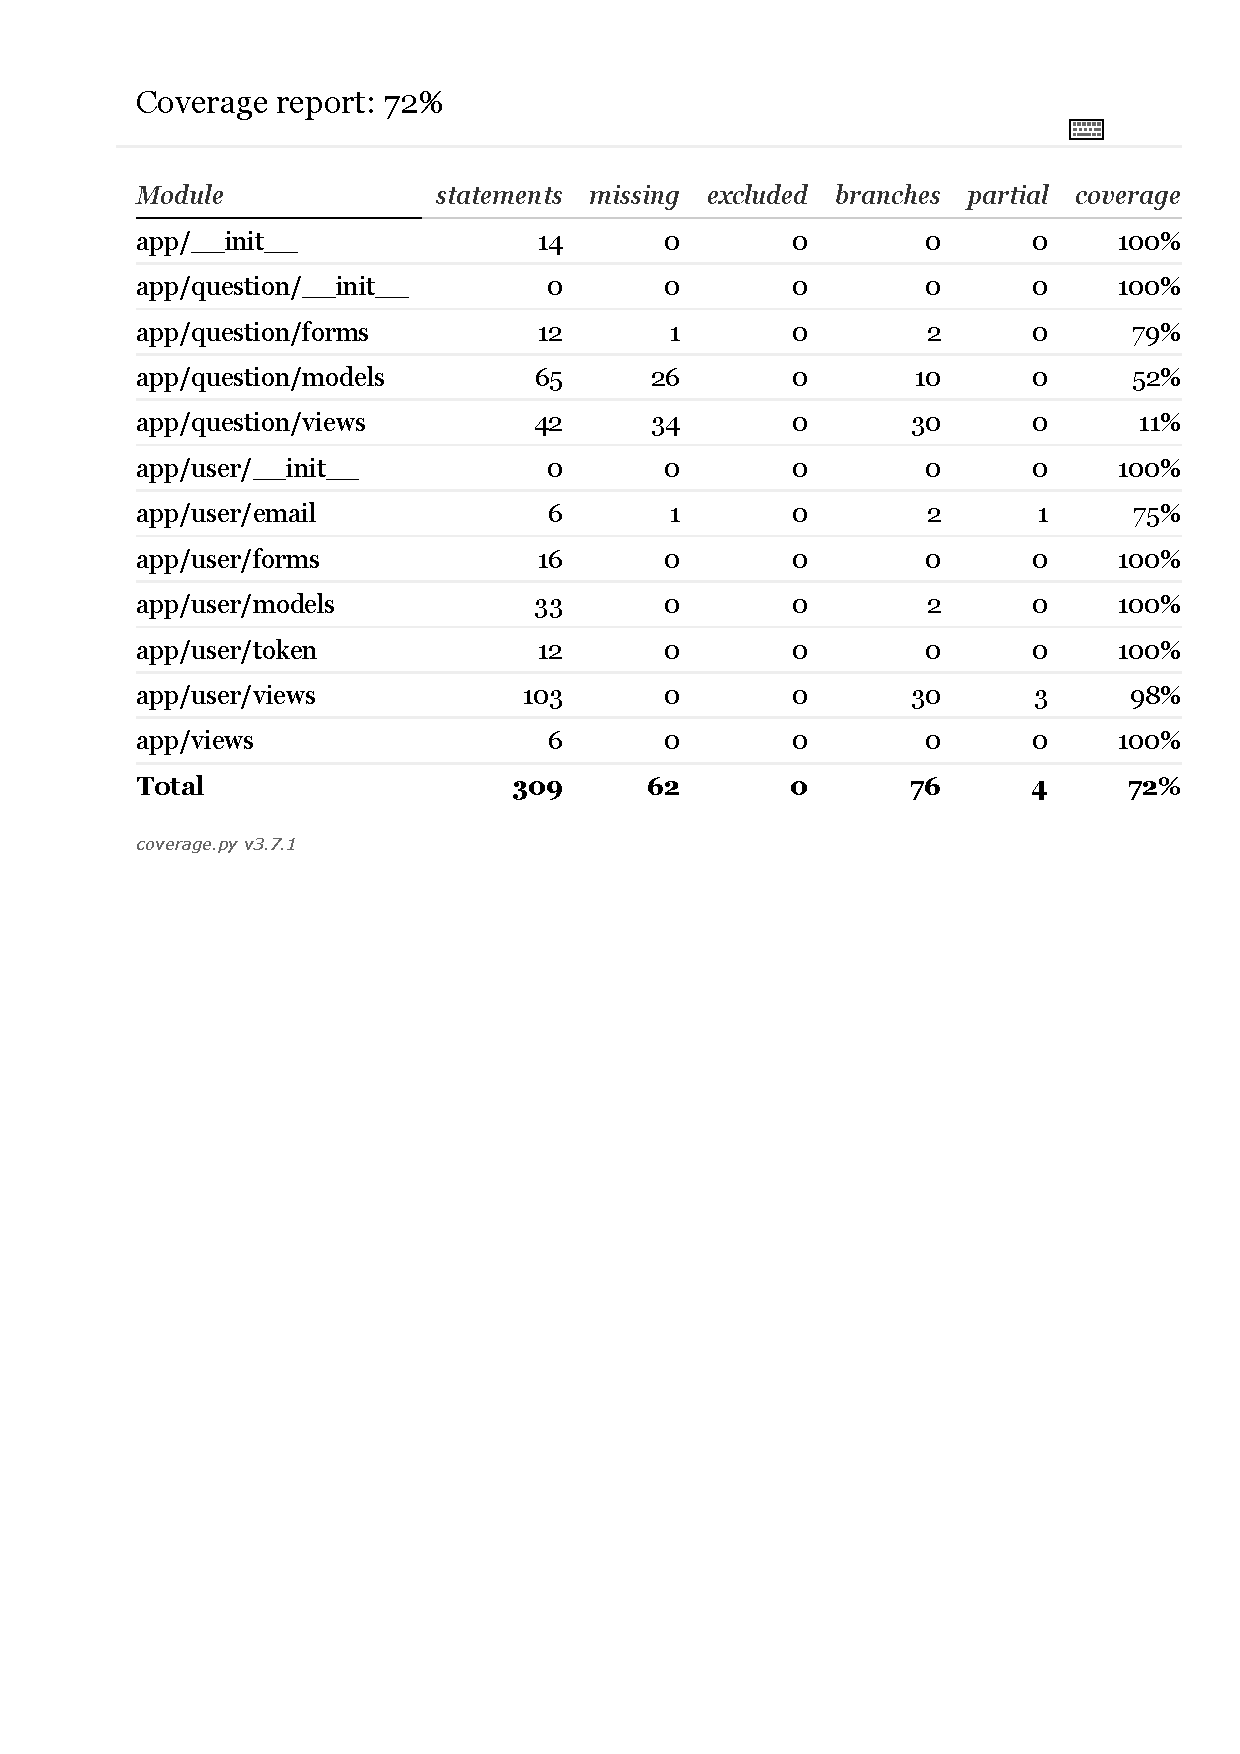
\includegraphics[width=0.8\linewidth]{figures/testcoverage.pdf}
    \caption{Oversigt over dækningsgraden af unittests. Det ses også hvor mange udtryk der er dækket af tests.}
    \label{fig:testcoverage}
\end{figure}

\begin{figure}[h]
    \centering
    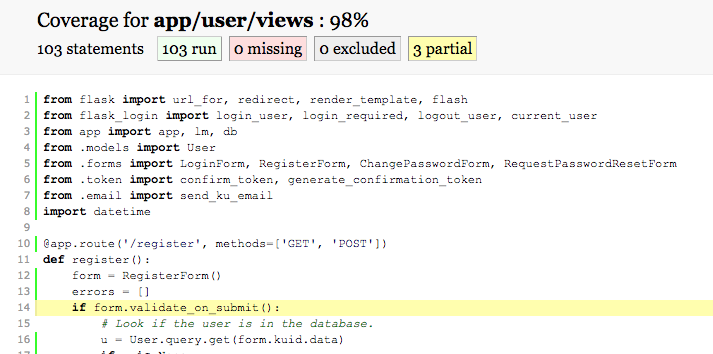
\includegraphics[width=0.8\linewidth]{figures/code_coverage.png}
    \caption{Eksempel på en grafik fremstilling, hvor et udtryk der kun delvist er dækket af tests fremhæves.}
    \label{fig:code_coverage}
\end{figure}

\section{Brugergrænseflade og interaktionsdesign}
\label{sec:brugergraenseflade}
\subsection{Screenshots}
I Appendix \ref{sec:screenshots} ses screenshots af brugergrænsefladen for de vigtigste dele af vores projekt. De optræder i en rækkefølge der illustrerer dynamikken i en studerendes interaktion med vores system. I toppen af de fleste screenshots ses en navigationsbar, hvor man bl.a. kan se hvem der er logget ind, man kan logge ud og man kan ændre sit password. Der er desuden i venstre side et slags logo hvor man kan trykke for at blive taget tilbage til forsiden.

På Figur \ref{fig:screenshot_login} ses et screenshot af den første del af vores brugergrænseflade en studerende vil møde, nemlig en login skærm. Hvis man allerede er registreret som bruger kan man her indtaste sit ku-id og sit valgte kodekord, og dermed logge på systemet. Hvis man ikke er oprettet som bruger er der et link der tager en videre til registrering. 

På Figur \ref{fig:screenshot_register} ses registreringssiden. Her kan man indtaste sit ku-id, vælge sig et kodeord og registrere sig. Systemet sender så en mail til den relevante ku-mail med et verificeringslink, og så snart den studerende har trykket på linket er vedkommende klar til at logge på systemet.

Når en studerende har logget sig ind i systemet vil vedkommende blive taget til index siden, som kan ses på Figur \ref{fig:screenshot_overview}. Her kan den studerende få et overblik over de forskellige \emph{thresholds} og de dertil hørende \emph{subjects}. Den studerende kan så vælge hvilket emne han vil arbejde på og klikke på dets navn, hvilket fører ham videre til den næste del.

På Figur \ref{fig:screenshot_subject} ses \emph{subject} siden, hvor den studerende kan læse om det valgte emne, og hvis det virker interessant, trykke på knappen og begynde at løse opgaver inden for det bestemte emne. De dummy-data vi har i databasen på nuværende tidspunkt er lidt simple, så derfor ser siden også lidt kedelig ud lige nu.

Når den studerende har trykket \emph{begin} vil vedkommende blive stillet en række opgaver, f.eks. multiple choice opgaver som den der kan ses på Figur \ref{fig:screenshot_question}. Den studerende kan så afgive sit svar, enten ved at indtaste et svar, afkryde de korrekte bokse eller trække svarmulighederne hen på de korrekte positioner, og trykke på \emph{answer} knappen. Der er desuden mulighed for at den studerende kan få hints til opgaven, hvis det skulle være nødvendigt, ved at trykke på den dertilhørende knap.

Når den studerende har svaret på en opgave vil vedkommende blive taget til svar-siden, som kan ses på Figur \ref{fig:screenshot_answer}. Her får den studerende feedback på sit svar, der kan variere fra en helt simpel besked i form af rigtigt eller forkert til et mere detaljeret svar der f.eks. kunne indeholde en relevant stack trace. På svar-siden er der desuden et såkaldt \emph{Learn-O-Meter}, hvor den studerende kan se hvor langt vedkommende er nået med at gennemføre det valgte emne.

Endeligt vil den studerende når vedkommende har gennemført et emne blive taget til en sidste side, som kan ses på Figur \ref{fig:screenshot_finish}, hvor der som det ser ud lige nu ikke står meget andet end \emph{Done}. Den studerende kan så trykke på \emph{finish} knappen, hvilket vil tage vedkommende til index siden, og derfra kan vedkommende så vælge et nyt emne at arbejde på, eller vælge at logge ud.

\subsection{Tænke-højt forsøg}
Vi har endnu ikke foretaget nogen tænke-højt forsøg. De tænkte brugere af vores system er i første omgang næste års nye studerende på datalogi uddannelsen, hvilket gør det svært for os at få fat i nogen af dem da de endnu ikke er startet. Omvendt er vi jo selv startet på datalogi for ikke så længe siden, så vi kunne muligvis godt gennemføre tænke-højt forsøg med nogle af vores medstuderende der ikke kender til vores system. Det har vi dog ikke gjort endnu, da vi først for nylig har fået færdiggjort en nogenlunde fungerende prototype og vi endnu ikke rigtig har nogen spørgsmål i databasen.

\section{Projektsamarbejdet}
\label{sec:projektsamarbejdet}
Samarbejdet med kunden fungerer stadig ganske udemærket. Når vi mødes med dem er der en meget afslappet og munter stemning, og det virker som om vi er meget godt på bølgelængde sammen og forstår at diskutere og blive enige om de forskellige aspekter af projektet. Vi er stadig ikke så gode til at være officielle og tage referater og den slags, mest fordi møderne mere er en mundtlig samtale og diskussion af projektet, og de ting vi bliver enige om er sjældent helt nye for os, så det er tanker vi allerede selv har gjort os. Vi har desuden endnu ikke haft en helt fungerende prototype at vise frem og bruge som basis for en mere konkret diskussion af projektet, men det skulle vi gerne have klar til næste gang vi skal mødes med kunden. 

Projektsamarbejdet internt i gruppen går nogenlunde, vi er ikke så gode til at holde sådan officielle møder  med dagsordener og referater og den slags, i stedet snakker vi bare sammen når vi lige mødes inde på universitetet, og arbejder på projektet når vi lige har tid, f.eks. i en pause eller en fri eftermiddag. Det meste af vores kommunikation foregår stadigvæk over email eller facebooks chat. 

Vi har for nyligt oprettet en to-do liste inde i vores git repository, hvor vi prøver at notere de forskellige ting ned der mangler at blive gjort, og som vi opdaterer løbende når vi får gennemført nogle af tingene eller støder på nye ting der skal laves. Det håber vi kan hjælpe os til at have et bedre overblik over projektet, og til at ikke glemme alle de små ting man måske støder på. På to-do listen er der tre sektioner, én til de store, vigtige ting, én til de mindre, mindre vigtige ting, og én til de ting der har at gøre med rapporten.

\newpage
\appendix
\section{Versionsstyring}
\label{sec:versionsstyring}
Link til github: \url{https://github.com/christiankjaer/pop-webhelp}
Siden sidste rapport har der været en del ændringer og især tilføjelser til koden. Vi har fået bundet alle de dele vi tidligere har lavet sammen til en fungerende prototype, der fungerer efter hensigten og som kan ses på de vedlagte screenshots. Derudover er vi begyndt at arbejde på admin delen af projektet, hvor mange af de overordnede aspekter er ved at være på plads.

\section{Changelog}
\label{sec:changelog}
\begin{tabular}{l l l}
08-04-2015 & CKL & Dokument oprettet. \\
14-04-2015 & CKL & Tilføjet use cases og krav. \\
16-04-2015 & LSE & Tilføjet UseCaseModel og BCE model. \\
16-04-2015 & CKL & Tilføjet review af Parnas og Clements. \\
17-04-2015 & TSH & Tilføjet review af Gould og Lewis. \\
17-04-2015 & LSE & Tilføjet Abstract og Projektsamarbejdet. \\
17-04-2015 & CKL & Tilføjet use cases, sekvensdiagram og klassediagram. \\
26-04-2015 & CKL & Tilføjet afsnit om tests. \\
30-04-2015 & CKL & Rettet til genaflevering og tilføjet systemdesign. \\
08-05-2015 & CKL & Tilføjet afsnit om strukturering. \\
10-05-2015 & LSE & Tilføjet Brugergrænseflade og screenshots, opdateret Systemdesign. \\
11-05-2015 & CKL & Tilføjet review af \cite{nsbullet}. \\
\end{tabular}

\section{Timeline}
\label{sec:timeline}
\begin{tabular}{l l p{8cm}}
11-03-2015 & Første møde med kunde: & Vi har første møde med kunden hvor vi snakker om hvad projektet går ud på og diskuterer krav og løsningsforslag. \\
16-04-2015 & Andet møde med kunde: & Vi har haft andet møde med kunden, hvor vi har snakket om modellen for de opgaver der skal være i systemet. \\
22-04-2015 & Internt møde i gruppen: & Vi har diskuteret databasemodeller, og vi er kommet frem til et databaseskema for denne iteration af systemet. Derudover fik vi udviklet i fællesskab på systemet. \\
27-04-2015 & Tredje møde med kunde: & Vi blev enige om en endelig funktionalitet for den første iteration af produktet. Derudover diskuterede vi udformingen af spørgmsålstyper og hvordan det hele skulle knyttes sammen. \\
07-05-2015 & Internt møde i gruppen: & Vi mødtes internt i gruppen for at diskutere udestående implementationsopgaver, og kigge på nogle ting sammen. \\
07-05-2015 & Første fungerende prototype & Vores første fungerende prototype af vores projekt er færdig, hvor vi har fået bundet alle de elementer vi løbende har lavet sammen til et sammenhængende hele. \\
\end{tabular}

\bibliographystyle{alpha}
\bibliography{refs}{}

\newpage
\section{ER-diagrammer}
\label{sec:er_diagrams}
\begin{figure}[h!]
    \centering
    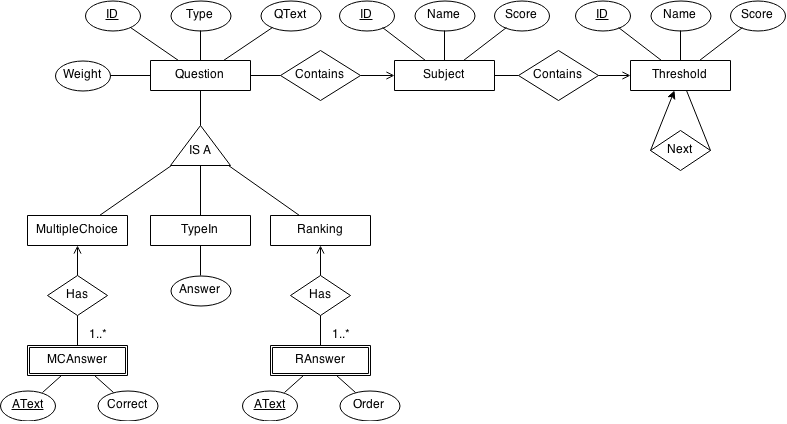
\includegraphics[width=0.8\linewidth]{figures/er_diagram/Qdb.png}
    \caption{ER-diagram over delen af databasen hvor spørgsmålene hører til.}
    \label{fig:er_diagram_question}
\end{figure}

\begin{figure}[h!]
    \centering
    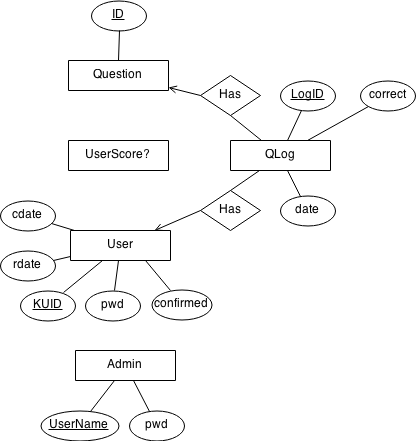
\includegraphics[width=0.8\linewidth]{figures/er_diagram/Logdb.png}
    \caption{ER-diagram over delen af databasen hvor loggen hører til.}
    \label{fig:er_diagram_log}
\end{figure}

\begin{figure}[h!]
    \centering
    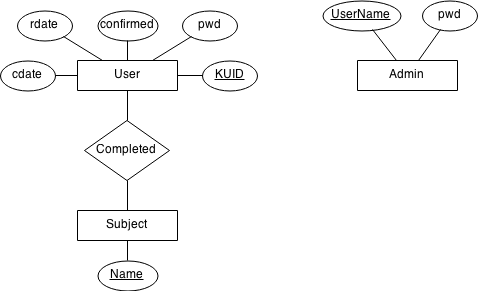
\includegraphics[width=0.8\linewidth]{figures/er_diagram/User.png}
    \caption{ER-diagram over delen af databasen hvor brugere og admins hører til.}
    \label{fig:er_diagram_user}
\end{figure}

\newpage
\section{Brugergrænseflade screenshots}
\label{sec:screenshots}
\begin{figure}[h!]
    \centering
    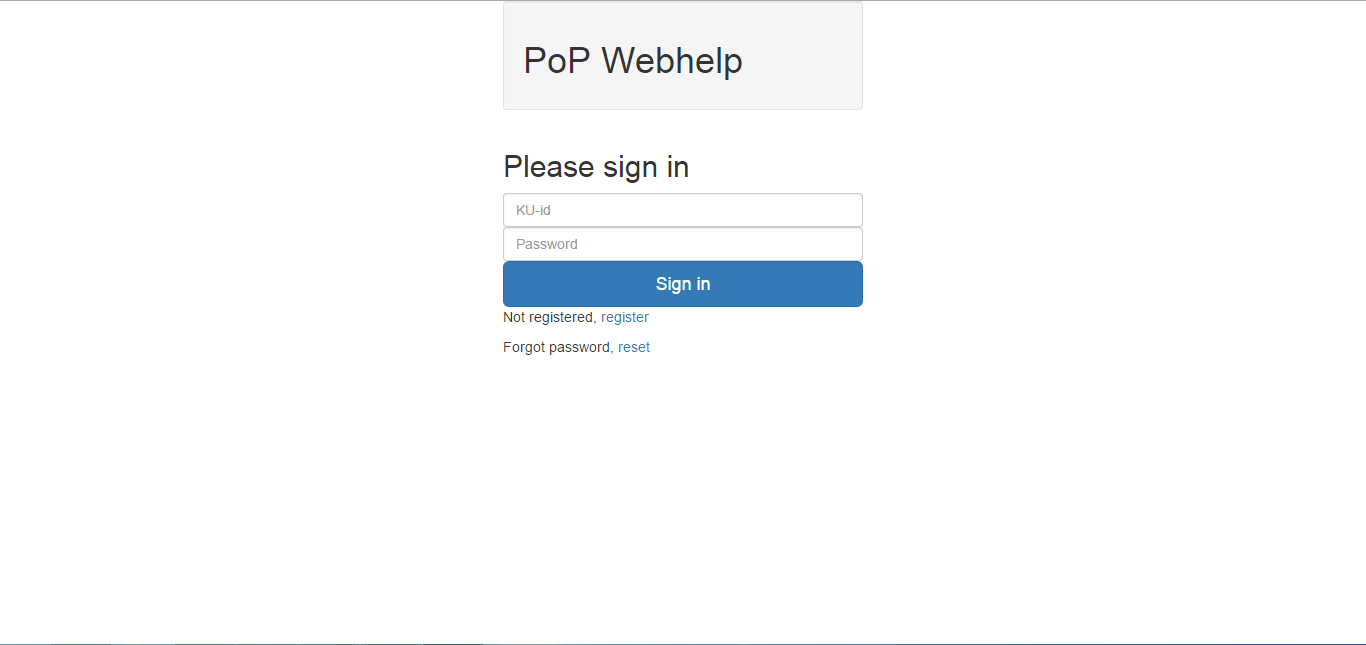
\includegraphics[width=1\linewidth]{figures/interface/login.png}
    \caption{Screenshot af login-siden.}
    \label{fig:screenshot_login}
\end{figure}


\begin{figure}[h!]
    \centering
    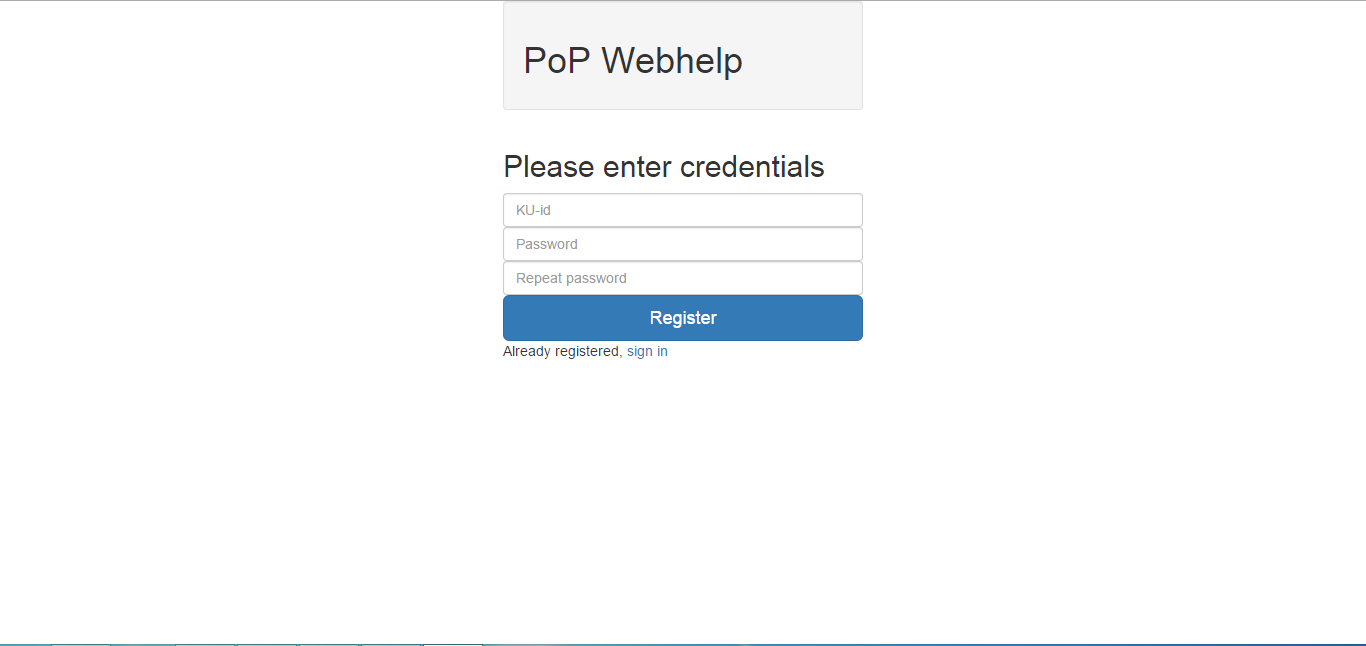
\includegraphics[width=1\linewidth]{figures/interface/register.png}
    \caption{Screenshot af registrerings-siden.}
    \label{fig:screenshot_register}
\end{figure}


\begin{figure}[h!]
    \centering
    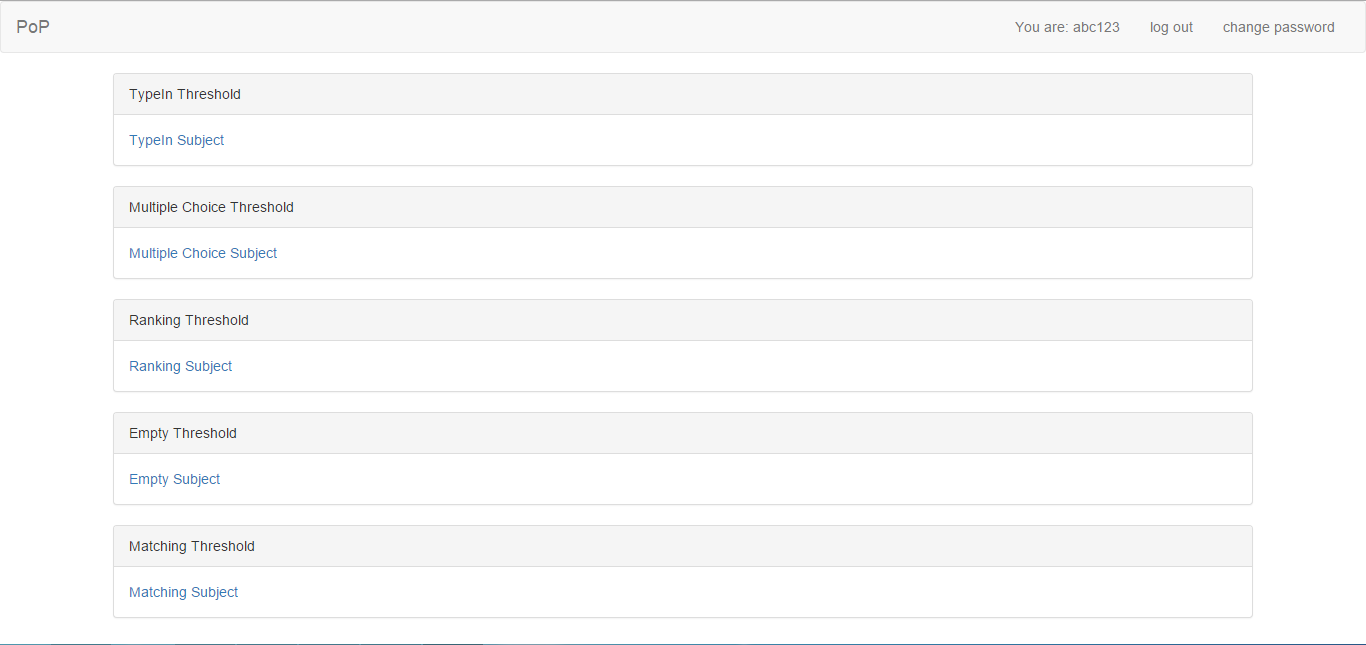
\includegraphics[width=1\linewidth]{figures/interface/overview.png}
    \caption{Screenshot af index-siden.}
    \label{fig:screenshot_overview}
\end{figure}


\begin{figure}[h!]
    \centering
    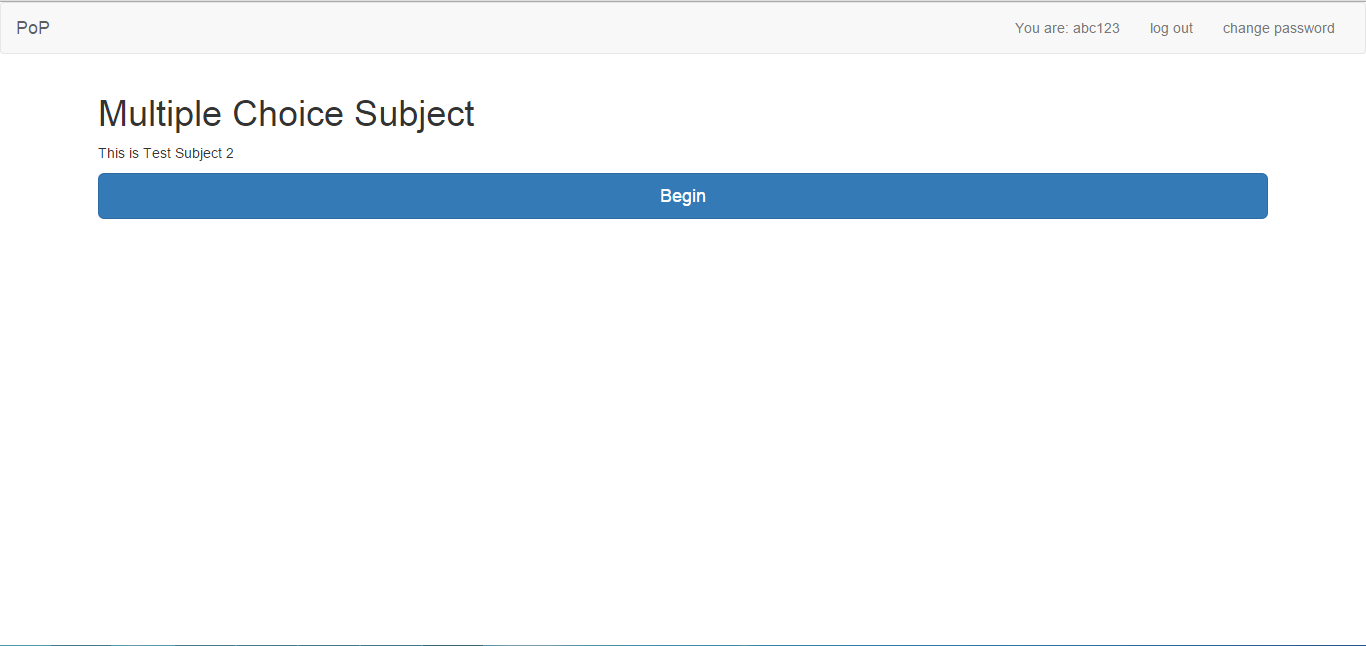
\includegraphics[width=1\linewidth]{figures/interface/subject.png}
    \caption{Screenshot af emne-siden.}
    \label{fig:screenshot_subject}
\end{figure}


\begin{figure}[h!]
    \centering
    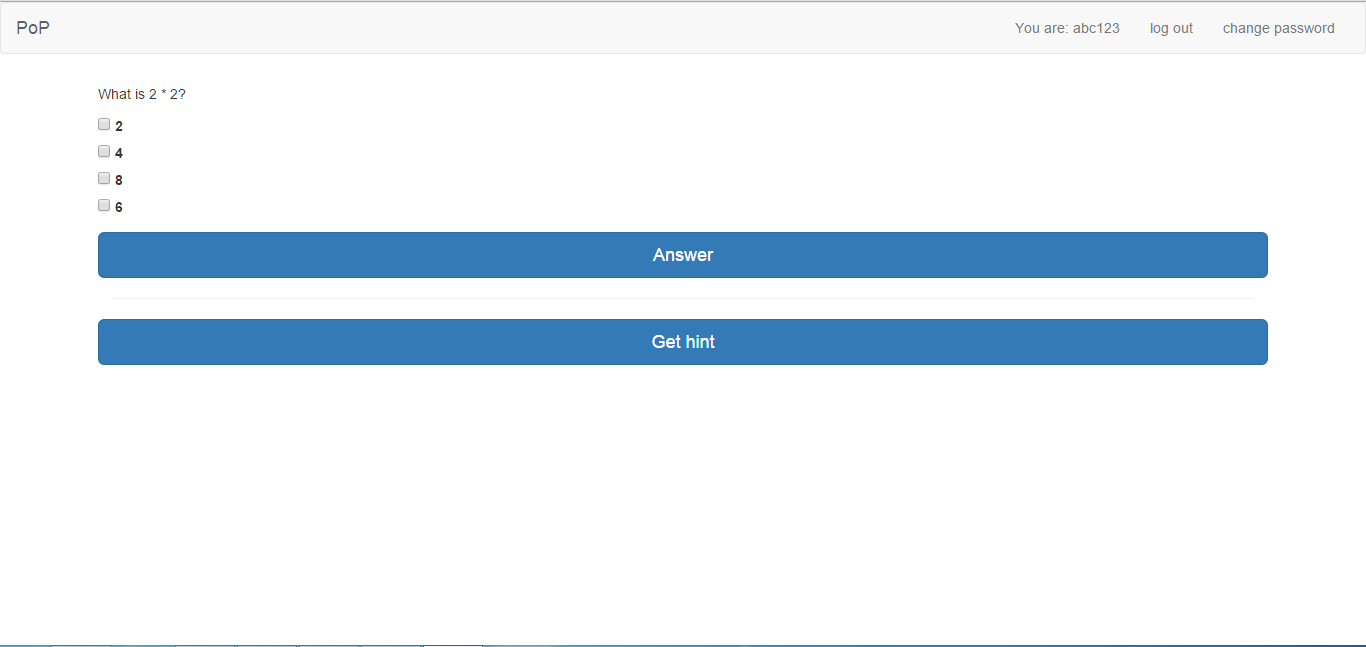
\includegraphics[width=1\linewidth]{figures/interface/question.png}
    \caption{Screenshot af spørgsmåls-siden.}
    \label{fig:screenshot_question}
\end{figure}


\begin{figure}[h!]
    \centering
    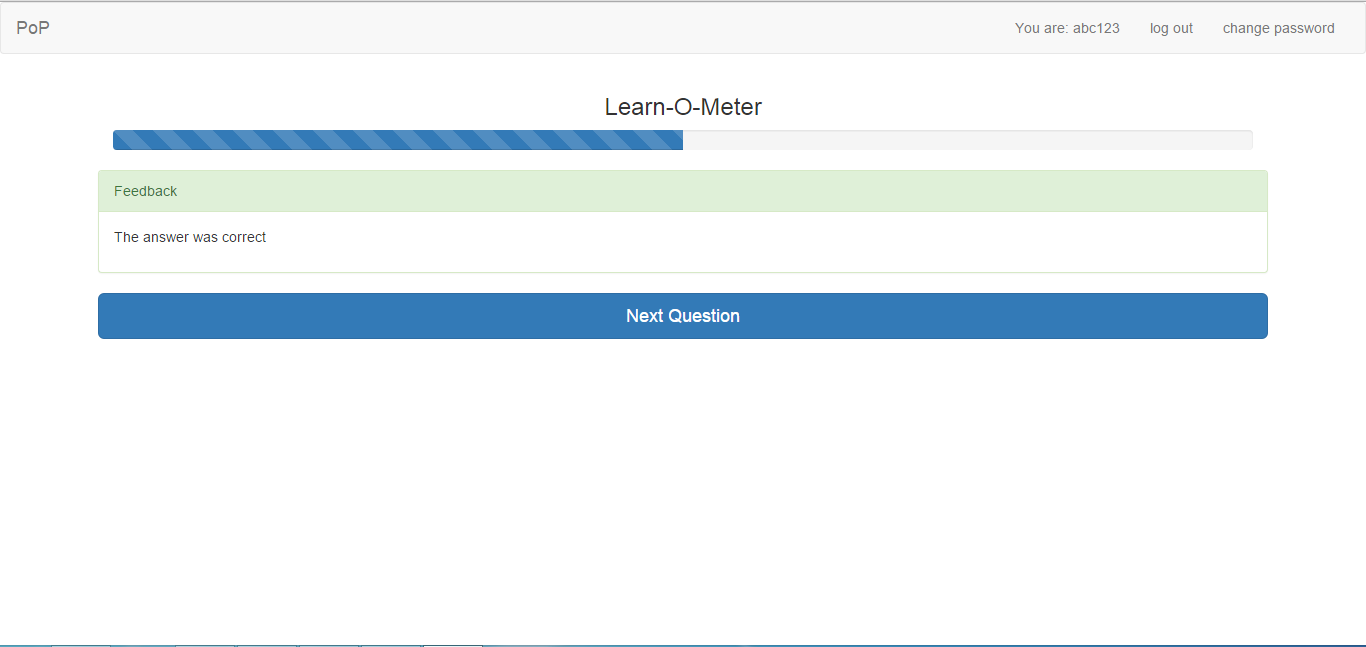
\includegraphics[width=1\linewidth]{figures/interface/answer.png}
    \caption{Screenshot af svar-siden.}
    \label{fig:screenshot_answer}
\end{figure}


\begin{figure}[h!]
    \centering
    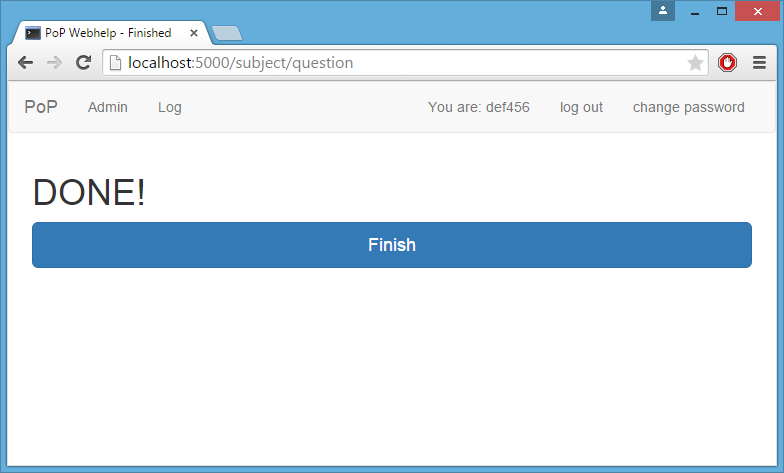
\includegraphics[width=1\linewidth]{figures/interface/finish.png}
    \caption{Screenshot af færdig-siden.}
    \label{fig:screenshot_finish}
\end{figure}

\end{document}
